
%\documentclass[12pt]{report}

\documentclass[12pt]{article}
%\usepackage{natbib}  % used for citations
\usepackage[parfill]{parskip} %used for formatting style of text



\usepackage{graphicx,fancyhdr}
\usepackage{amssymb,amsmath}
\usepackage{epigraph,fancyvrb,eqparbox}
\usepackage[multiple]{footmisc}
\usepackage{menukeys}
\usepackage{menukeys}
\usepackage{url}
\usepackage[colorlinks = true, linkcolor = blue, urlcolor = blue]{hyperref}
\usepackage{setspace}

\pagestyle{fancyplain}

%\usepackage{hyperref}
%\usepackage{epsf,psfig,graphicx,fancyheadings}
% \textwidth 7in
% \textheight 9in
% \oddsidemargin 0in
% \topmargin -.25in

%-----------------------------------------------
% The following settings are from Dr. Davidian's
% ST810A Handout on Advanced LaTeX Features

%\setlength{\paperheight}{11.0in}
%\setlength{\paperwidth}{8.5in}

%%%%%%%%%%%%%%%%%%%%%%%%%%%%%%%%%%%%%%%%%%%%%%%%%
% For Desktop @ CalPoly (for Postscript)

%\setlength{\oddsidemargin}{0.5in}
%\setlength{\evensidemargin}{0.5in}
%\setlength{\topmargin}{-.5in}

%%%%%%%%%%%%%%%%%%%%%%%%%%%%%%%%%%%%%%%%%%%%%%%%%
% For Laptop @ Calpoly (for Postscript)

% \setlength{\oddsidemargin}{0.in}
% \setlength{\evensidemargin}{0.in}
% \setlength{\topmargin}{0.25in}

%%%%%%%%%%%%%%%%%%%%%%%%%%%%%%%%%%%%%%%%%%%%%%%%%
% For Desktop @ CalPoly (for PDF)

%\setlength{\oddsidemargin}{0.in}
%\setlength{\evensidemargin}{0.in}
%\setlength{\topmargin}{-.5in}
%
%%%%%%%%%%%%%%%%%%%%%%%%%%%%%%%%%%%%%%%%%%%%%%%%%%
%% For Laptop @ Calpoly (for PDF)
%
%% \setlength{\oddsidemargin}{0.in}
%% \setlength{\evensidemargin}{0.in}
%% \setlength{\topmargin}{0.25in}
%
%
%
%\setlength{\oddsidemargin}{0.0in}
%\setlength{\topmargin}{-0.5in}
%\setlength{\headheight}{0.20in}
%\setlength{\headsep}{3ex}
%\setlength{\baselineskip}{2ex}
%\setlength{\textheight}{9in}
%\setlength{\textwidth}{6.4in}
%\renewcommand{\baselinestretch}{1.1}

% Sets margins to 1 in
\addtolength{\oddsidemargin}{-.5in}%
\addtolength{\evensidemargin}{-.5in}%
\addtolength{\textwidth}{1in}%
\addtolength{\textheight}{1.3in}%
\addtolength{\topmargin}{-.8in}%

%\setlength{\headheight}{0.20in}
%\setlength{\headsep}{3ex}
%\setlength{\headrulewidth}{0.2pt}
%\setlength{\footrulewidth}{0.15pt}
%\setlength{\parskip}{2.3ex}
% %set to no indentation
%\setlength{\parindent}{0.0in}
%\setlength{\baselineskip}{2ex}
%\setlength{\textheight}{9.in}
%\setlength{\textwidth}{6.5in}

\def \doublespace{\openup 2\jot}
% For double or 1.5 spacing
%\renewcommand{\baselinestretch}{1.5}
\tolerance=500

\def\boxit#1{\vbox{\hrule\hbox{\vrule\kern6pt
\vbox{\kern6pt#1\kern6pt}\kern6pt\vrule}\hrule}}
\renewcommand{\theequation}{\thesection.\arabic{equation}}
% The following for TOC
%\renewcommand{\thepage}{\roman{page}}
% to be followed by this for the main text
\renewcommand{\thepage}{\arabic{page}}


%-----------------------------------------------

%%%%%%%%%%%%%%%%%%%%%%%%%%%%%%%%%%%%%%
%Define any shortcut aliases below

\newtheorem{theo}{Theorem}[section]

\newenvironment{note}{\begin{quote}\emph{Note:\ }}{\end{quote}}
\newenvironment{defn}{
\begin{description}
\item[Definition ]}
{\end{description}}

\newenvironment{ttscript}[1]{%
    \begin{list}{}{%
    \settowidth{\labelwidth}{\texttt{#1}}
    \setlength{\leftmargin}{\labelwidth}
    \addtolength{\leftmargin}{\labelsep}
    \setlength{\parsep}{0.5ex plus0.2ex minus0.2ex}
    \setlength{\itemsep}{0.3ex}
    \renewcommand{\makelabel}[1]{\texttt{##1\hfill}}}}
    {\end{list}}

\newcommand{\bt}{\begin{tabular}}
\newcommand{\et}{\end{tabular}}
\newcommand{\bc}{\begin{center}}
\newcommand{\ec}{\end{center}}
\newcommand{\bi}{\begin{itemize}}
\newcommand{\ei}{\end{itemize}}
\newcommand{\be}{\begin{enumerate}}
\newcommand{\ee}{\end{enumerate}}
\newcommand{\bq}{\begin{quote}}
\newcommand{\eq}{\end{quote}}
\newcommand{\vect}[1]{\mbox{\boldmath $ #1$}}
\newcommand{\avg}[1]{$\overline{#1}$}
\newcommand{\bmp}{\begin{minipage}}
\newcommand{\emp}{\end{minipage}}
\newcommand{\hr}{\u{\hspace{7in}}}
\newcommand{\sr}{\u{\hspace{5in}}}
\newcommand{\chs}{\chi^2}

\newcommand{\labn}[1]{\Large{\textbf{\fbox{Lab #1}}}\hspace{0.1in} \normalsize{\emph{Some of these problems may be more challenging than others. Please feel free to work with others, attend office hours, or post on the course discussion forum if you need help.  While collaboration with other students is encouraged, each student is responsible for submitting his or her own work.  This assignment should be submitted in one well-commented SAS program.  For any questions that require a written answer, do so in the SAS comments.  Be sure to re-name the uploaded SAS scripts according to the naming convention}} \texttt{LastnameFirstinitial\textunderscore Lab\#.sas} (\emph{e.g.,} \texttt{PileggiS\textunderscore Lab#1.sas}).}


\newcommand{\hd}[1]{\lhead{STAT 330/530: Lab #1}\rhead{Pileggi, FA17}}
\newcommand{\bs}{\underline{\hspace{0.5in}}}

%\newcommand{\bv}{\footnotesize
%\bmp{.5\textwidth}
%\begin{Verbatim}[frame=single,label=SAS Code,commandchars=\\\{\}],xrightmargin=.5\textwidth}
%
%\newcommand{\ev}{\end{Verbatim}
%\emp
%\normalsize}

\newcommand{\bv}{\begin{code}}
\newcommand{\ev}{\end{code}}

 \newenvironment{code}[1]%
  {\vspace{.1in}\footnotesize\Verbatim[frame=single,label=SAS Code,commandchars=\\\{\},xrightmargin=#1\textwidth,framesep=.2in,labelposition=all]}
  {\endVerbatim\normalsize}

\newenvironment{craw}[2]%
{\vspace{.1in}\footnotesize\Verbatim[frame=single,label=#2,commandchars=\\\{\},xrightmargin=#1\textwidth,framesep=.2in,labelposition=all]}
  {\endVerbatim\normalsize}

\newenvironment{cbox}[1]%
{\vspace{.1in}\footnotesize\Verbatim[frame=single,commandchars=\\\{\},xrightmargin=#1\textwidth,framesep=.2in,labelposition=all]}
  {\endVerbatim\normalsize}

\newcommand{\head}[1]{\large \textbf{#1} \normalsize}

\newcommand{\ttt}[1]{\textbf{\texttt{#1}}}


\newcommand{\bsval}[1]{\underline{\hspace{0.2in}{[#1]}\hspace{0.2in}}}

\newcommand{\ttb}{\textbf}
\newcommand{\tte}{\emph}
\newcommand{\ttu}{\underline}



\newcommand{\jdhr}{\vspace{0.2in}\hrule}


\newcommand{\uspace}[1]{\underline{\hspace{#1}}}

\newenvironment{ident}{\begin{list}{}{}
         \item[]}{\end{list}}

\newenvironment{proposition}{
\begin{description}
\item[Proposition: ]}
{\end{description}}

\newcommand{\bpr}{\begin{proposition}}
\newcommand{\epr}{\end{proposition}}



% \newenvironment{example}
%     {
%         \begin{list}{\textbf{Example:}}
%         {
%         \settowidth{\labelwidth}{}
%         \setlength{\leftmargin}{\labelwidth}
%         }
%     }
%     {\end{list}}


\newenvironment{example}{
\jdhr \vspace{-.17in}\jdhr
\textbf{Example: }}
{}

\newcommand{\bex}{\begin{example}}
\newcommand{\eex}{\end{example}}

\newenvironment{onyourown}{
\jdhr \vspace{-.17in}\jdhr
\textbf{On Your Own: }}
{}

\newcommand{\boy}{\begin{onyourown}}
\newcommand{\eoy}{\end{onyourown}}


%\newenvironment{debug}{
%\jdhr \vspace{-.17in}\jdhr
%\ttb{Debug the Code}
%\fbox{
%\bmp{.95in}
%\includegraphics[height=.35in]{C:/images/bug4.jpg}\includegraphics[height=.35in]{C:/images/buggy8.jpg}
%\emp}
%}
%{\jdhr}

\newenvironment{debug}{
\jdhr \vspace{-.17in}\jdhr
\ttb{Debug the Code: }
\fbox{
\bmp{.95in}
\includegraphics[height=.35in]{C:/images/bug4.jpg}\includegraphics[height=.35in]{C:/images/mushi90.jpg}
\emp}
}
{}


\newcommand{\bbug}{\begin{debug}}
\newcommand{\ebug}{\end{debug}}


\begingroup
  \catcode `_=11
  \gdef\myuscore{_}
  \catcode `~=11
  \gdef\mytilde{~}
  \catcode `\|=0
  \catcode `\\=11
  |gdef|mybs{\}
|endgroup

%Define any shortcut aliases above


%....................................................................
%....................................................................
%....................................................................
%....................................................................
%....................................................................
%....................................................................
%....................................................................
%....................................................................



\usepackage{amssymb}
				




\begin{document}
\hd{9}
\labn{9}

\noindent The following data sets contain student information for an introductory statistics course.  The course had one large lecture and 12 smaller lab sections.  There are 14 data sets as follows:
\begin{itemize}
\item \ttt{LE1}, \ttt{LE2}, ... \ttt{LE12} contains information from the official course rosters for the 12 lab sections, downloaded on the first day of class
\item \ttt{survey} contains information asked in a course survey in the first week of class, and contains background information about the students
\item \ttt{grades} is a record of the student grades at the end of the quarter
\end{itemize}
\noindent You may use as many data steps and/or procs as needed to achieve the following objectives.
\begin{enumerate}
\item Create a macro variable called \ttt{path} that corresponds to the computer location of these data sets.
\item Write a macro to import the 14 data sets into SAS (you should use your \ttt{path} macro variable).
\item Combine all 14 data sets.
\item Create a variable called \ttt{type} that classifies students as follows:
\item[]
\begin{enumerate}
\item \ttt{dropped} - these students were present on the official course roster, but not present in the grades data set
\item \ttt{crashed} - these students were not present on the official course roster, but present in the grades data set
\item \ttt{no survey} - these students are present on the official course roster and have grades, but did not fill out the survey
\item \ttt{complete} - these students are present on the official course roster, have survey responses, and have grades
\end{enumerate}
\item Identify the number of students in each classification of the \ttt{type} variable.  Your results should match those below.
\item[]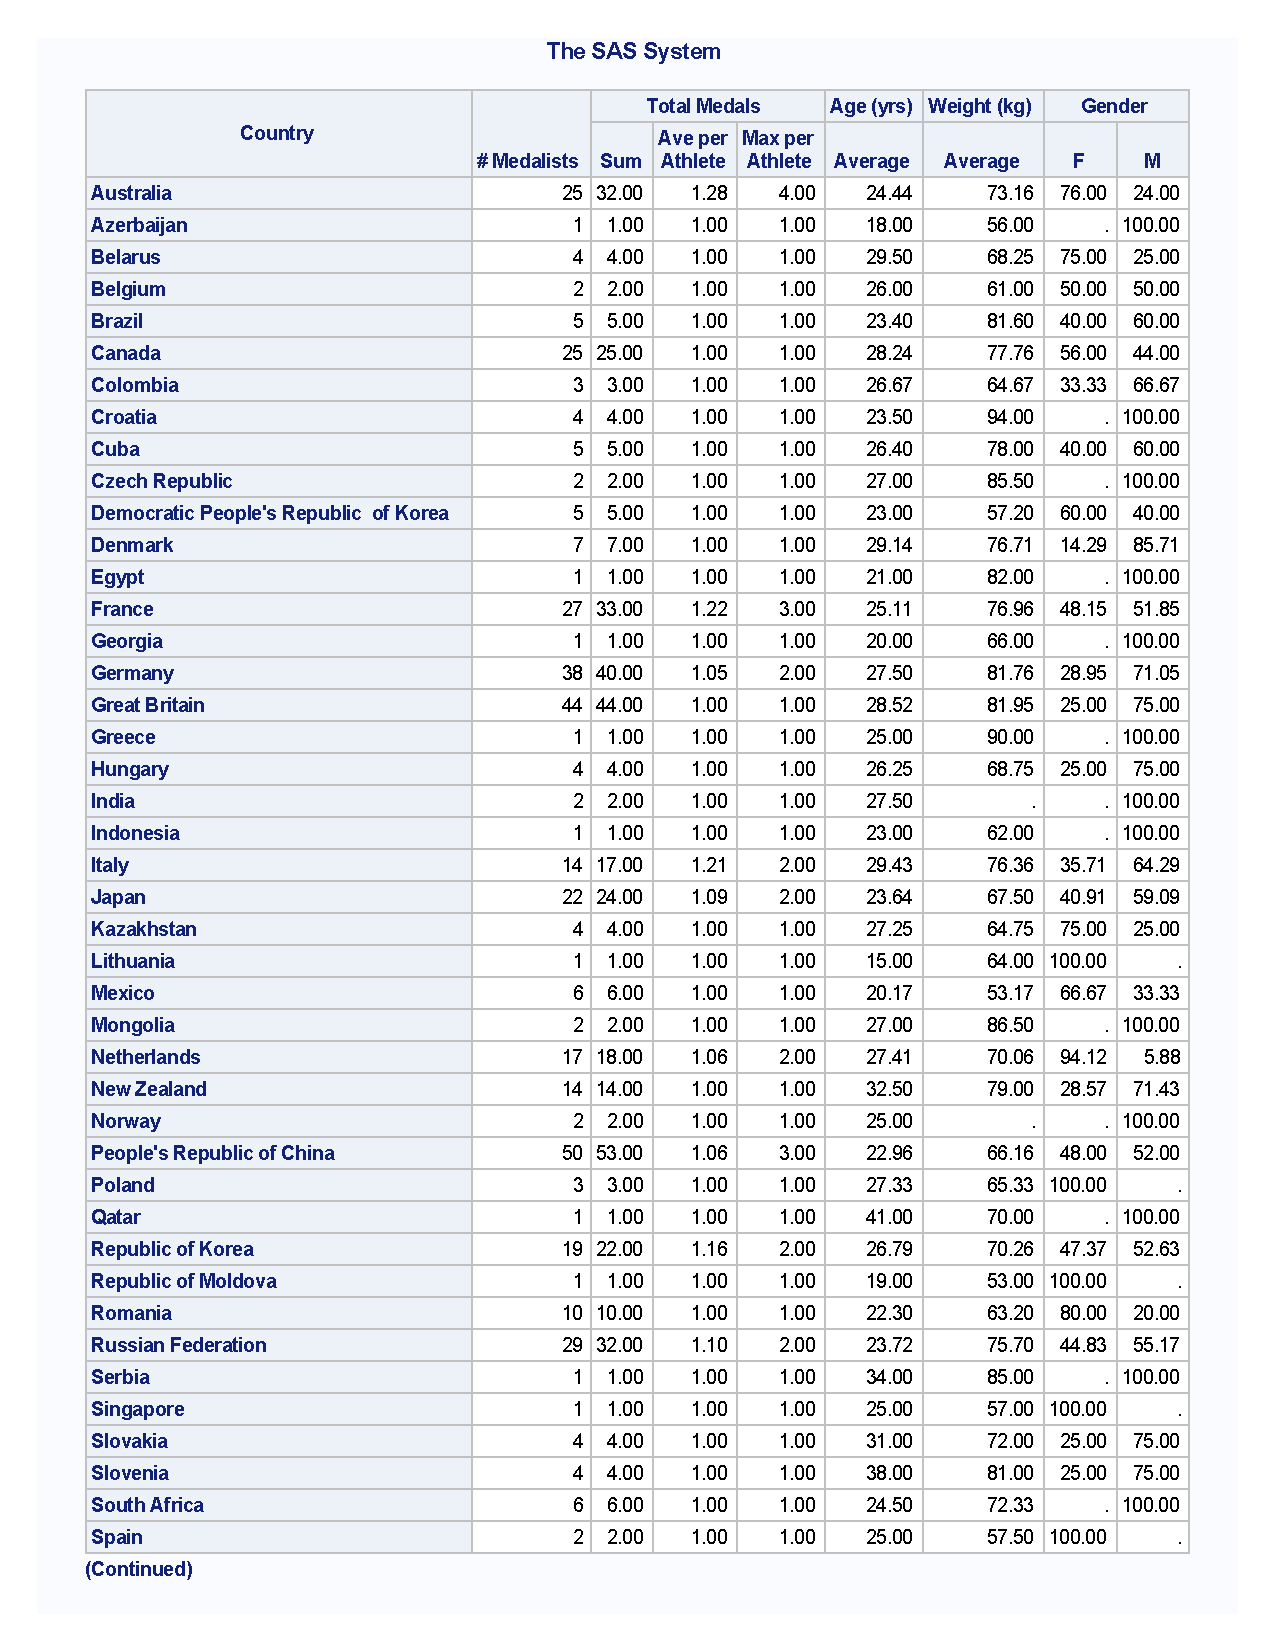
\includegraphics[trim={6cm 23.0cm 6cm 1.3cm},clip]{q5.pdf}
\item Create a data set that removes the students who dropped.  Use this data set for the remaining exercises.
\item All recorded grades are presented in terms of percents.  However, the grading rubric was in terms of points.  There was a miscommunication on one of the lab assignments where the grader accidentally entered too many points, and so the grade recorded as over 100\%.  Use a SAS procedure to identify the \textbf{lab assignment(s)} that has(have) incorrect grades (ie, do not figure this out by viewing/scanning the data). Note that on homeworks and exams students could earn some extra credit, so grades may be over 100\% on those assignments.  Verify that your re-coding was done correctly.
\item Re-code the \textbf{lab assignment(s)} with values exceeding 100 percent to be equal to 100 percent.  Verify that your re-coding was done correctly.
\item When entering grades for homeworks, labs, or quizzes, the TA entered \ttt{-99} for missing grades.  \ttb{Using arrays}, recode all values of \ttt{-99} to zero.   Verify that your re-coding was done correctly.
\item Calculate each student's average homework, lab, and quiz grade. (Note, there is no lab 1 grade.)  Also, calculate each student's overall course grade, weighted as follows:  homework 15\%, labs 15\%, quizzes 5\%, exam 1 20\%, exam 2 20\% and final exam 25\%.  Verify that your re-coding was done correctly.  The grade distribution should match that shown below.  
\item[]\item[]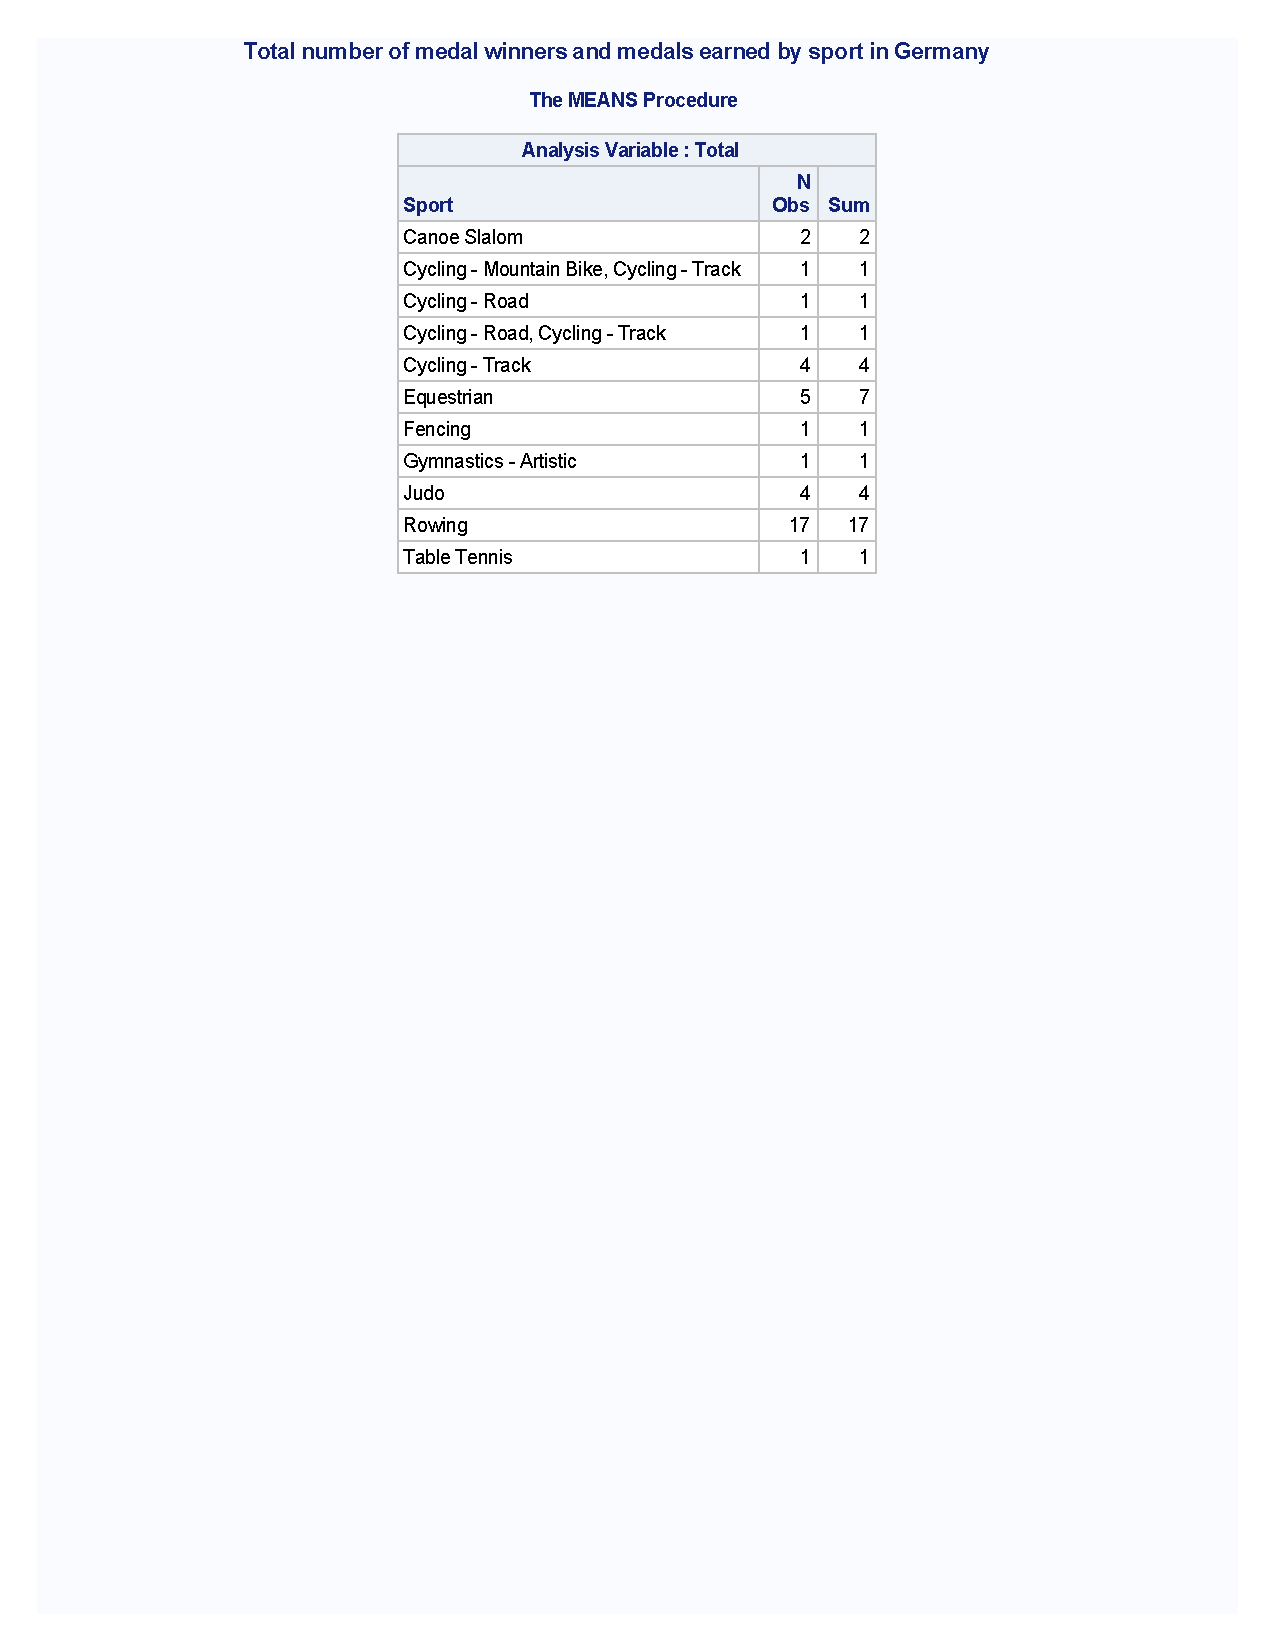
\includegraphics[trim={5cm 24.0cm 5cm 1.3cm},clip]{q10.pdf}
\item Create a new variable in the data set that represents the letter grade for each student such that A=90-100, B=80-89.9, C=70-79.9, D=60-70.9, F=0-59.9.  Some students didn't actually complete the course, and should get a letter grade of W for withdrawal.  These students can be identified as those that did not take the final exam and so have a grade of \ttt{0} for the final exam grade. Verify that your re-coding was done correctly.  The letter grade distribution should match that shown below.
\item[]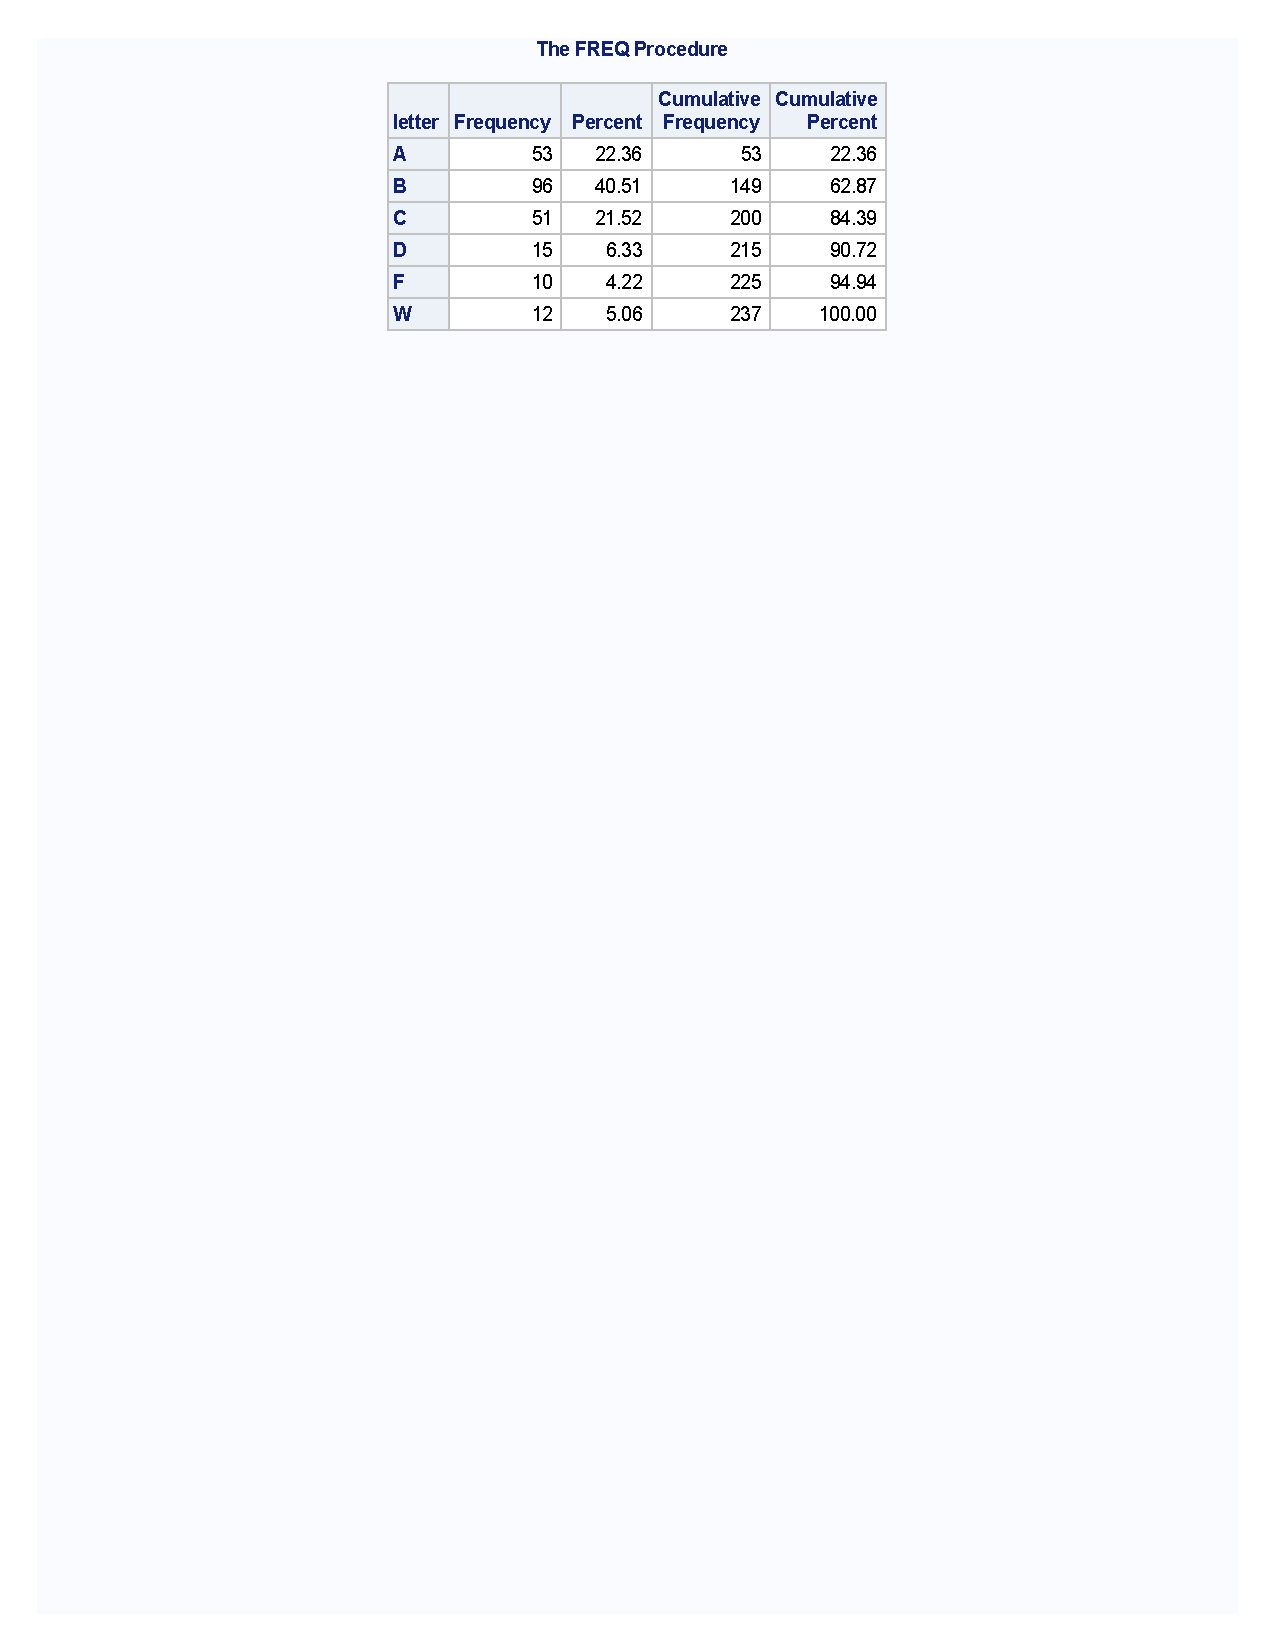
\includegraphics[trim={6cm 22.0cm 6cm 1.3cm},clip]{q11.pdf}
\item The professor wants to analyze grades by major.  Create a new variable called major that takes the classifications of undeclared, biology, psychology, and other.  Make sure that students who have a missing program and plan also have a missing value for major.  (Any program and plan that has the word ``Biology'' in it should be classified as a biology major.  Then create the following table that summarizes final course grade by major such that there are four rows corresponding to the four majors, and three columns corresponding to the sample size, the average course grade, and the standard deviation of course grade.  The results should match that shown below.
\item[]
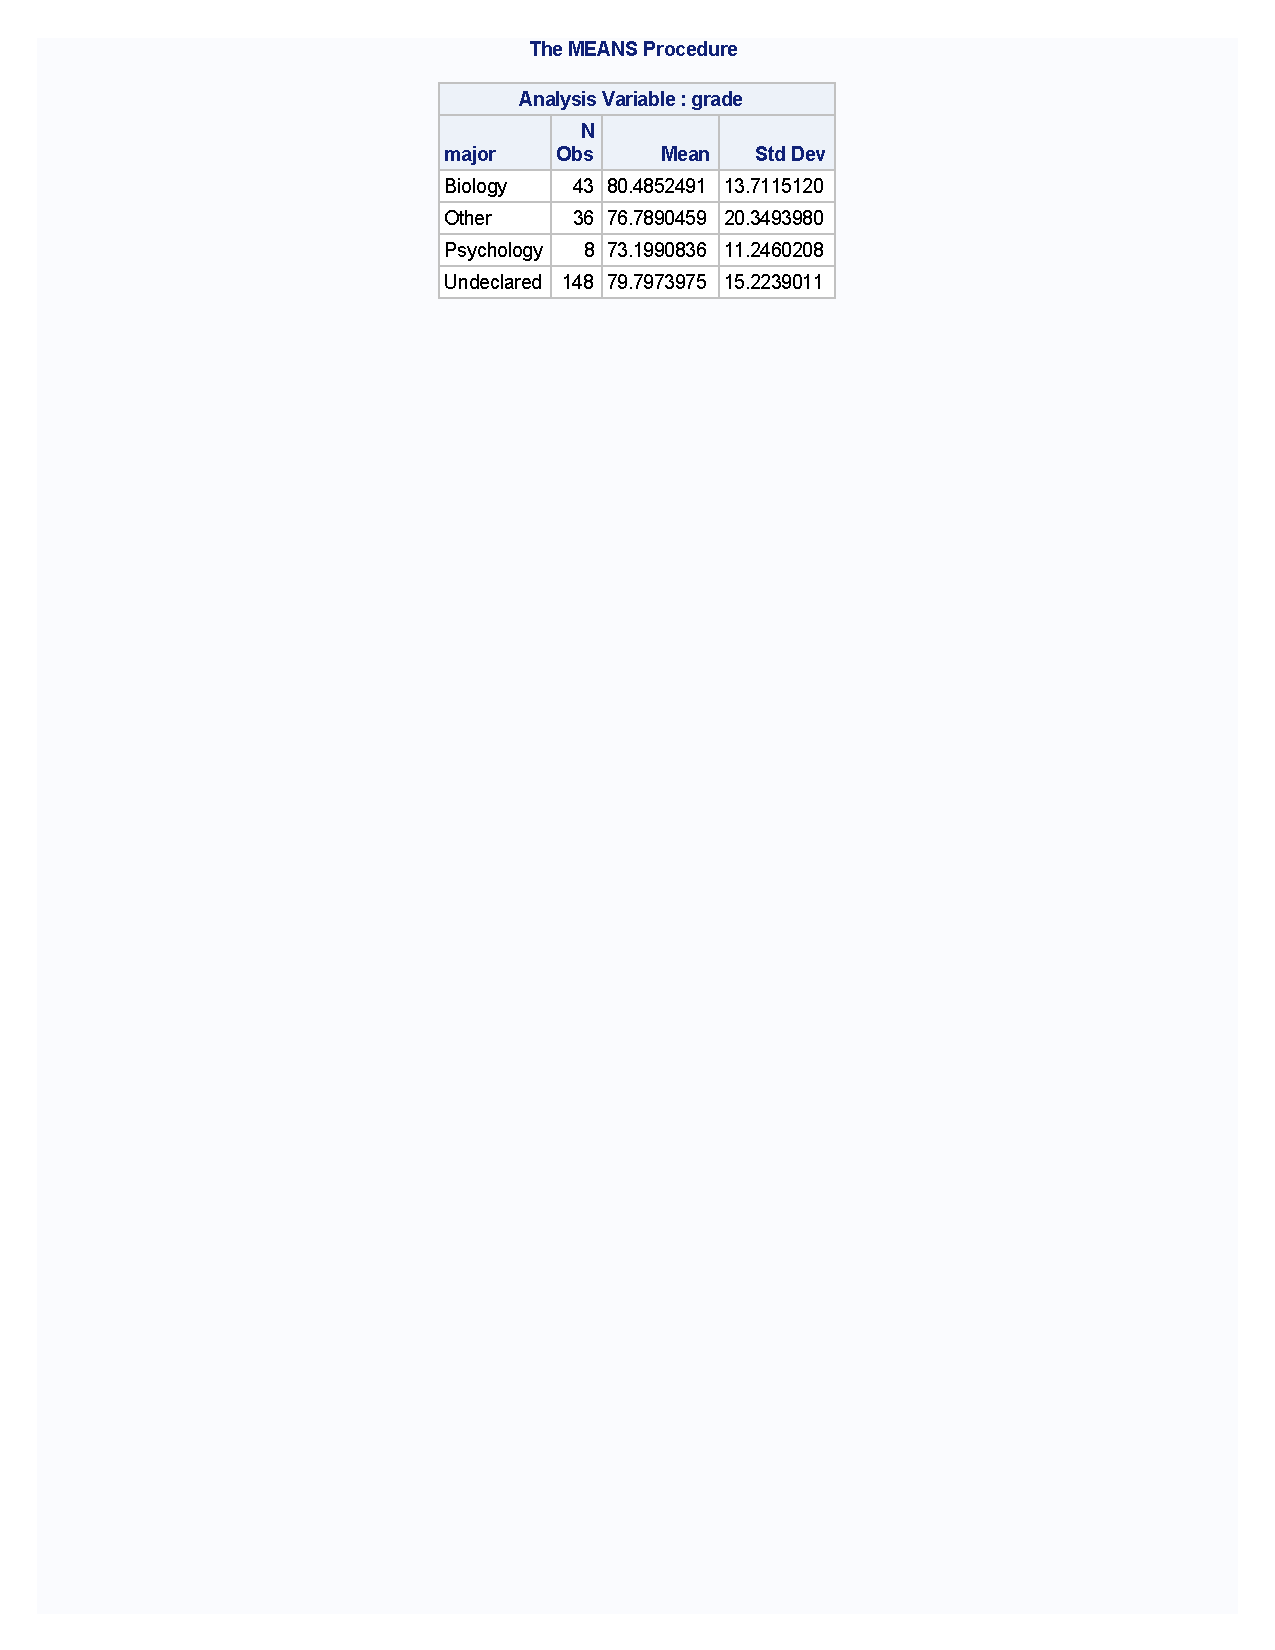
\includegraphics[trim={6cm 21.0cm 6cm 1.3cm},clip]{q12.pdf}
%\item Create the following table that summarizes final course grade by major such that there are four rows corresponding to the four majors, and three columns corresponding to the sample size, the average course grade, and the standard deviation of course grade.  Labels and formatting are not important.  Create this table three ways:
%\begin{enumerate}
%\item using \ttt{proc means}
%\item using \ttt{proc sql}
%\item using either \ttt{proc report} or \ttt{proc tabulate}
%\end{enumerate}
%\item[]
%\bmp{0.5\textwidth}
%\includegraphics[trim={6cm 21.0cm 6cm 1.3cm},clip,width=1.0\textwidth]{Lab18means.pdf}
%\includegraphics[trim={6.1cm 21.0cm 6.1cm 0.5cm},clip,width=1.0\textwidth]{Lab18tab.pdf}
%\emp
%\bmp{0.5\textwidth}
%\includegraphics[trim={6cm 22.0cm 6cm 0.5cm},clip,width=1.0\textwidth]{Lab18sql.pdf}
%\includegraphics[trim={6.1cm 21.0cm 6.1cm 0.5cm},clip,width=1.0\textwidth]{Lab18rep.pdf}
%\emp
%\item Suppose that the students in this class are representative of a larger population of students taking introductory statistics.  Professors want to know how exam 1 grade compares to exam 2 grade.  Perform a statistical test to determine if the population average exam grade changed between exam 1 and exam 2, and interpret your results.
%\item Suppose that the students in this class are representative of a larger population of students taking introductory statistics.  Professors want to know if intention to pursue a health related degree (\ttt{PreHealthN}) is related to the final course grade.  Perform a statistical test, and interpret your results.  (You do not need to re-code \ttt{PreHealthN}.)
\end{enumerate}
\end{document} 